\documentclass[hyperref=colorlinks]{beamer}
\mode<presentation>
\usetheme{iclpt}
\setbeamertemplate{navigation symbols}{}
\setbeamertemplate{headline}{
\begin{beamercolorbox}[leftskip=.2cm,rightskip=.2cm,topskip=.2cm,ht=1.1cm,dp=0.1cm,wd=\textwidth]{institute in head/foot}
  
\includegraphics[height=1cm]{icl.pdf}
  \hfill
  
\includegraphics[height=1cm]{../Pics/CMS-Color.pdf}
\end{beamercolorbox}
}
\setbeamertemplate{footline}{
\begin{beamercolorbox}[ht=.55cm,dp=0.4cm,wd=\textwidth,leftskip=.3cm]{author in head/foot}%
  \begin{minipage}[c]{5cm}%
    \usebeamerfont{author in head/foot}
    \insertshortauthor 
    \insertshorttitle
    \end{minipage}\hfill%
  \insertframenumber{} / \pageref{lastframe}
  \hfill
  \begin{minipage}{6cm}
    \hfill
  \end{minipage}
\end{beamercolorbox}%
}

\usepackage{color}
\usepackage{tabularx,colortbl}
\usepackage{graphicx}
\usepackage{pdfpages}
\usepackage{feynmp}
\DeclareGraphicsRule{*}{mps}{*}{}

\title{\vspace{-0.2cm} Progress with Limits}
%\subtitle{Paper - HIG-13-030, PASs: HIG-13-013, HIG-13-018, HIG-13-028 \vspace{-0.7cm}}
\author[P. Dunne]{\underline{P. Dunne} }%\\ on behalf of the H$\rightarrow$invisible analysis groups} % A.M. Magnan and A. Nikitenko Joao Pela with \\ R. Aggleton, J. Brooke: Bristol \\ C.Asawangtrakuldee, Q.Li: Peking \\ P. Srimanobhas: Chulalongkorn \\ S. Kumar, K. Mazumdar: Mumbai}
\titlegraphic{
  \vspace{-0.7cm}
  %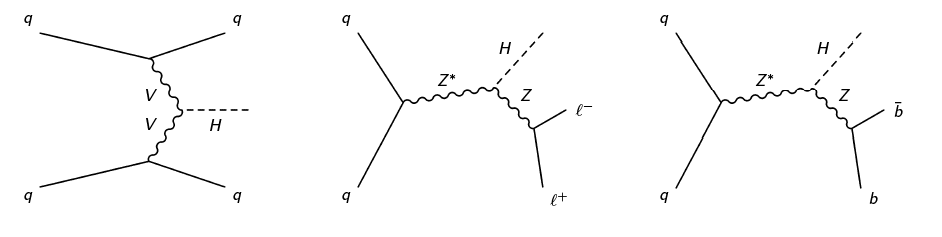
\includegraphics[width=\textwidth]{TalkPics/invcomb021213/feyndiags}
%% \begin{fmfgraph*}(100,70)
%%         \fmfleft{i1,i2}
%%         \fmfright{o1,o2,o3}
%%         \fmf{fermion}{i1,v1,o1}
%%         \fmf{fermion}{i2,v2,o3}
%%         \fmf{phantom,tension=4/5}{v1,v2}
%%         \fmffreeze
%%         \fmf{photon,label=$W,,Z$}{v1,v3}
%%         \fmf{photon,label=$W,,Z$}{v2,v3}
%%         \fmf{dashes}{v3,o2}
%%         \fmflabel{$q$}{i1}
%%         \fmflabel{$q$}{i2}
%%         \fmflabel{$q$}{o1}
%%         \fmflabel{$q$}{o3}
%%         \fmflabel{$H$}{o2}
%%       \end{fmfgraph*}
}
\date{}
\begin{document}
\begin{fmffile}{hig1330approvalfeynmandiags}

%TITLE PAGE
\section{Title}
\begin{frame}
  \titlepage
  
\end{frame}

%OUTLINE


\begin{frame}
  \frametitle{Reminder of last week}
    \begin{block}{}
      \scriptsize
      \begin{itemize}
      \item Most systematics now implemented:
      \item[-] Still missing: ggH theory uncertainties, WGamma cross section uncertainty, error on QCD contribution.
      \item Still currently ignoring QCD
      \item Had tried region with less QCD:
      \item[-] metsig$>4$, $min\Delta\phi(alljets,metnomu)>1.5$
      \item[-] expected limit: 0.9102
      \item Added mjj$>1000$ and CJV
      \item[-] expected limit: 0.5371
      \end{itemize}
    \end{block}
\end{frame}

\begin{frame}
  \frametitle{Updates}
  \begin{block}{}
    \scriptsize
    \begin{itemize}
    \item Top reweighting is now fully included, no noticeable change to expected limit
    \item Prompt selection has been applied to parked data
    \item[-] Expected limit 51\%, ignoring top and QCD
    \item[-] Worse limit seems to be due to fewer data events in Z control region
    \item Lxplus5 shut down, need to transfer limit code to IC SL5 machines
    \end{itemize}
  \end{block}
  
\end{frame}

\begin{frame}
  \frametitle{Scan through variables}
  \begin{columns}
    \column{1.1\textwidth}
    \begin{block}{}
      \scriptsize
      \begin{itemize}
      \item Have now also scanned through mjj, met significance and jetmetdphi cut
      \item Best working point found was metsig$>4$, mjj$>1000$, jetmetdphi$>2.5$
      \item[-] Expected limit: 0.2764
      \end{itemize}
      \begin{tabular}{|l||c|c||c|c|c|c|c|c|c||c|}
        \hline
        Process & ggH   &  qqH    & zvv   &  wmu   &  wel   &  wtau  &  top  &   wg    &  vv & total \\
        \hline
        Rate & 21.5  &  316.0& 143.8& 71.9& 47.7& 10.2& 4.4& 3.6& 5.4 & 287\\
        \hline
      \end{tabular}
      \begin{itemize}
      \item Weights for V+jets regions decrease further needs investigating
      \item[-] wenu: 0.32, wmunu: 0.38, wtau: 0 (clearly wrong), top: 0.55
      \item Limits ignoring systematics are 10.2\%, was 16.6\% for prompt
      \item 19 events in Z control region, was 12 for prompt
      \end{itemize}
    \end{block}
    \end{columns}
\end{frame}

\begin{frame}
  \frametitle{Uncertainty Impact Check- some low impact not listed}
  \begin{columns}
    \column{1.1\textwidth}
  \vspace{-.4cm}

  \begin{block}{}
    \scriptsize
    \begin{tabular}{|l|c|c|}
      \hline
      Nuisance & \% change from removal & \% change from addition \\
      \hline
CMS\_eff\_m:               &      -0.7\%          &                3.8\% \\
CMS\_scale\_j:             &      -2.8\%          &                3.8\% \\
CMS\_res\_j:               &       0.0\%          &                0.0\% \\
CMS\_scale\_met:            &      0.0\%           &               0.4\% \\
CMS\_VBFHinv\_puweight:    &      -4.3\%          &               29.6\% \\
CMS\_VBFHinv\_zvv\_norm:   &       -2.8\%         &                27.7\% \\
CMS\_VBFHinv\_zvv\_stat:   &      -15.6\%         &                84.1\% \\
CMS\_VBFHinv\_wmu\_norm:   &       -0.7\%         &                 4.7\% \\
CMS\_VBFHinv\_wmu\_stat:    &      -0.7\%         &                 3.8\% \\
CMS\_VBFHinv\_wel\_norm:    &      -0.7\%         &                 4.7\% \\
CMS\_VBFHinv\_wel\_stat:    &      -1.4\%         &                 6.7\% \\
CMS\_VBFHinv\_tau\_eff:     &       0.0\%         &                 0.0\% \\
CMS\_VBFHinv\_wtau\_norm:   &       0.0\%         &                18.1\% \\
CMS\_VBFHinv\_wtau\_stat:   &       0.0\%         &                17.1\% \\
CMS\_VBFHinv\_zvv\_extrapfacunc:&  -9.2\%        &                 63.1\% \\
CMS\_VBFHinv\_top\_norm:        &   0.0\%        &                  0.0\% \\
CMS\_VBFHinv\_top\_stat:     &      0.0\%        &                  0.9\% \\
      \hline
    \end{tabular}
  \end{block}
  \end{columns}
\end{frame}

\begin{frame}
  \frametitle{The Wtau problem}
  \begin{block}{}
    \scriptsize
    \begin{itemize}
    \item W tau background weight is concerning
    \item[-] Only 2 events in data control region
    \item Added top reweighting and NCBkg became larger than NCData
    \item First remove CJV from all categories
    \item[-] Limit improved by a couple of percent on removal, seems redundant
    \item Doesn't change number of data events in tau control region
    \end{itemize}
  \end{block}
\end{frame}

\begin{frame}
  \frametitle{Loosening jet met dphi}
  \begin{columns}
  \column{1.09\textwidth}
  \begin{columns}    
    \column{.55\textwidth}
  \begin{block}{}
    \scriptsize
    \begin{itemize}
    \item Next step: try loosening jetmetdphi cut in tau control region
      \end{itemize}
      \begin{tabular}{|l|c|c|c|}
        \hline
        Cut & NCData & NSMC & Exp. Limit \\
        \hline
        $>$1.0 & 24 & $118\pm 32 \pm 24$ & 0.3926 \\
        $>$0.0 & 136 & $118\pm 12\pm 10$ & 0.2803 \\
        \hline
      \end{tabular}
      \begin{itemize}
    \item Is this extrapolation valid?
    \item[-] Check difference in munu shape where we have enough events
    \item Weight changes from 0.48 to 0.39 when cut loosened to 1.0
    \item Apply a 20\% systematic to WTau estimate to account for this
    \item[-] Expected limit goes to 0.2998
    \end{itemize}
  \end{block}
  \column{.45\textwidth}
  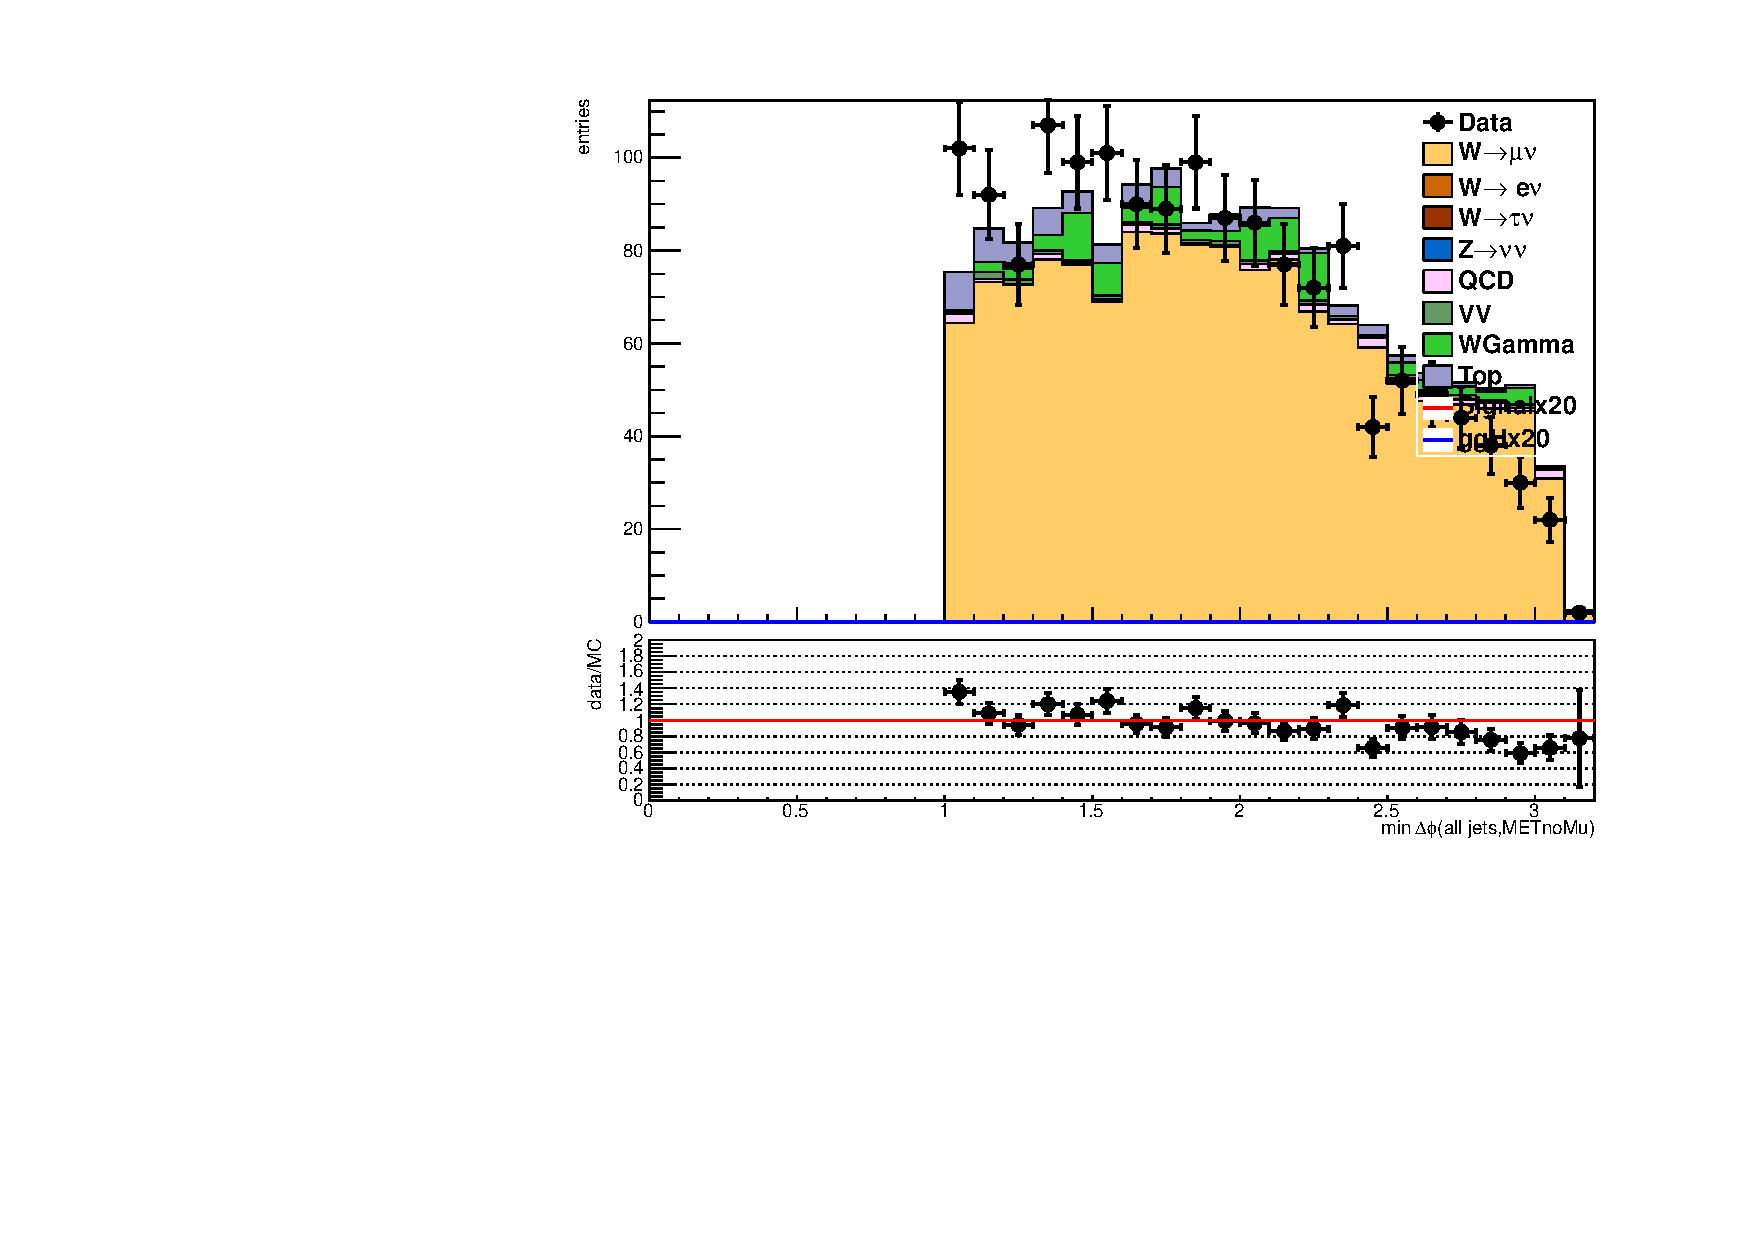
\includegraphics[width=\textwidth,height=.7\textheight]{TalkPics/limits131014/munu_alljetsmetnomu_mindphi.pdf}
  \end{columns}
  \end{columns}
\end{frame}

%WTAU CUT LOOSENING EFFECT
%jobs_alljets10loosertaunocjvmetsig4mjj1000/ no taunu jetmetdphi cut
%jobs_alljets25loosertaunocjvmetsig4mjj1000/ no taunu jetmetdphi cut
%jobs_alljets25loosetaunocjvmetsig4mjj1000/  taunu jetmetdphi>1.0 cut
%jobs_alljets25tighttaunocjvmetsig4mjj1000/  taunu jetmetdphi>2.5 cut

\begin{frame}
  \frametitle{Conclusions}
  \label{lastframe}

  \begin{block}{}
    \scriptsize
    \begin{itemize}
    \item Next steps: BDT
    \item More work to be done on trigger weights
    \item Anne Marie raised the point that our W+jets and WGamma samples may overlap
    \item[-] Filter has been added to light tree maker, will be applied next time light trees are remade
    \end{itemize}
  \end{block}

\end{frame}

\begin{frame}
  \frametitle{Backup}
\end{frame}

\begin{frame}
  \frametitle{First try at limits}
  \begin{columns}
    \column{1.1\textwidth}
  \begin{block}{}
    \scriptsize
    \begin{itemize}
    \item Haven't fixed on QCD estimation method yet:
    \item[-] Pick region where QCD small/negligible
    \item[-] metsig$>4$, $min\Delta\phi(alljets,metnomu)>1.5$
    \item Rates:
    \end{itemize}
    \begin{tabular}{|l||c|c||c|c|c|c|c|c|c||c|}
      \hline
      Process & ggH   &  qqH    & zvv   &  wmu   &  wel   &  wtau  &  top  &   wg    &  vv & total bkg \\
      \hline
      Rate & 146 & 930 & 1065 & 670 & 467 & 1207 & 76 & 84 & 41 & 3610\\
      \hline
    \end{tabular}
    \begin{itemize}
      \item Expected Limit: 0.9102
      \item[-] Prompt expected was 0.49
      \item Wtau is dominant background
    \end{itemize}
  \end{block}
  \end{columns}
\end{frame}

\begin{frame}
  \frametitle{Uncertainty Impact Check - Impacts above 0.5\%}
  \begin{columns}
    \column{1.1\textwidth}
  \vspace{-.4cm}

  \begin{block}{}
    \scriptsize
    \begin{tabular}{|l|c|c|}
      \hline
      Nuisance & \% change from removal & \% change from addition \\
      \hline
      lumi\_8TeV:            &         -0.9\%     &                     0.0\% \\
      CMS\_eff\_e:                &     -0.9\%         &                 3.5\% \\
      CMS\_eff\_m:                &     -0.9\%         &                13.3\% \\
      CMS\_scale\_j:              &    -28.1\%         &               487.0\% \\
      CMS\_res\_j:                &     -2.6\%         &               121.2\% \\
      CMS\_scale\_met:            &     -0.9\%         &                13.3\% \\
      CMS\_VBFHinv\_puweight:     &     -0.9\%         &                48.6\% \\
      CMS\_VBFHinv\_zvv\_norm:     &     -0.9\%         &                23.8\% \\ 
      CMS\_VBFHinv\_zvv\_stat:     &     -2.6\%         &                86.0\% \\
      CMS\_VBFHinv\_wmu\_norm:     &     -0.9\%         &                 3.5\% \\
      CMS\_VBFHinv\_wmu\_stat:     &     -0.9\%         &                 3.5\% \\
      CMS\_VBFHinv\_wel\_norm:     &     -0.9\%         &                 3.5\% \\
      CMS\_VBFHinv\_wel\_stat:     &     -0.9\%         &                 7.9\% \\
      CMS\_VBFHinv\_tau\_eff:      &     -0.9\%         &                74.9\% \\
      CMS\_VBFHinv\_wtau\_norm:    &     -3.4\%         &               175.9\% \\
      CMS\_VBFHinv\_wtau\_stat:    &     -5.2\%         &               234.0\% \\
      CMS\_VBFHinv\_zvv\_extrapfacunc: & -8.6\%         &               188.2\% \\
      pdf\_qqbar:                &     -0.9\%         &                 0.0\% \\
      \hline
    \end{tabular}
  \end{block}
  \end{columns}
\end{frame}

\begin{frame}
  \frametitle{Scanned through variables}
  \begin{columns}
    \column{1.1\textwidth}
    \begin{block}{}
      \scriptsize
      \begin{itemize}
      \item Add CJV
      \item[-] Expected limit: 0.7090
      \end{itemize}
      \begin{tabular}{|l||c|c||c|c|c|c|c|c|c||c|}
        \hline
        Process & ggH   &  qqH    & zvv   &  wmu   &  wel   &  wtau  &  top  &   wg    &  vv & total \\
        \hline
        Rate & 115 & 880& 909 &510 &342 &886 &41 &67& 29 & 2783\\
        \hline
      \end{tabular}
      \begin{itemize}
      \item Add CJV and mjj$>1000$
      \item[-] Expected limit: 0.5371
      \end{itemize}
      \begin{tabular}{|l||c|c||c|c|c|c|c|c|c||c|}
        \hline
        Process & ggH   &  qqH    & zvv   &  wmu   &  wel   &  wtau  &  top  &   wg    &  vv & total\\
        \hline
        Rate & 68 & 668 & 457 & 291 & 192 & 285 & 17 & 32 & 15 & 1288\\
        \hline
      \end{tabular}
    \end{block}
    \end{columns}
\end{frame}

\begin{frame}
  \frametitle{Uncertainty Impact Check - cjv mjj1000}
  \begin{columns}
    \column{1.1\textwidth}
    \vspace{-.4cm}
    \begin{block}{}
      \scriptsize
       \begin{tabular}{|l|c|c|}
         \hline
         Nuisance & \% change from removal & \% change from addition \\
         \hline
         lumi\_8TeV:               &      -0.7\%        &                  0.5\%  \\
         CMS\_eff\_m:              &       -0.7\%       &                   8.0\% \\
         CMS\_scale\_j:            &      -23.3\%       &                 289.8\% \\
         CMS\_res\_j:              &       -0.7\%       &                  30.1\% \\
         CMS\_VBFHinv\_puweight:   &       -0.7\%       &                  23.0\% \\
         CMS\_VBFHinv\_zvv\_norm:  &        -0.7\%      &                   22.1\% \\
         CMS\_VBFHinv\_zvv\_stat:  &        -5.1\%      &                   85.4\% \\
         CMS\_VBFHinv\_wmu\_norm:  &        -0.7\%      &                    5.0\% \\
         CMS\_VBFHinv\_wmu\_stat:  &        -0.7\%      &                    5.0\% \\
         CMS\_VBFHinv\_wel\_norm:  &        -0.7\%      &                    5.0\% \\
         CMS\_VBFHinv\_wel\_stat:  &        -0.7\%      &                    8.0\% \\
         CMS\_VBFHinv\_wtau\_norm: &        -2.2\%      &                  116.0\% \\
         CMS\_VBFHinv\_wtau\_stat: &        -2.9\%      &                  144.1\% \\
         CMS\_VBFHinv\_zvv\_extrapfacunc:&  -9.5\%      &                  120.1\% \\
         CMS\_VBFHinv\_top\_stat:  &        -0.4\%      &                    2.0\% \\
         pdf\_qqbar:               &      -0.4\%        &                  0.0\% \\
         \hline
       \end{tabular}
    \end{block}
  \end{columns}
\end{frame}





\end{fmffile}
\end{document}
